\chapter{内核、Boot和printf}

\section{实验目的}
  \begin{enumerate}
    \item 掌握操作系统实验所需的基本工具
    \item 从操作系统角度理解MIPS体系结构
    \item 掌握操作系统启动的基本流程
  \end{enumerate}
在本章中,我们需要阅读并填写部分代码,使得我们的小操作系统可以正常的运行起来。这一章节的难度较为简单,
主要是为了让大家熟悉操作系统实验环境中的各类工具,为后续的实验奠定基础。
    
\section{操作系统的启动}

\subsection{内核在哪里?}
通过《计算机组成原理》课的学习,我们知道计算机是由硬件和软件组成的,仅有一个裸机是什么也干不了的;
另一方面,软件也必须运行在硬件之上才能实现其价值。由此可见,硬件和软件是相互依存、密不可分的。
为了能较好的管理计算机系统的硬件资源,我们需要使用操作系统。
而操作系统本身也是一种软件,我们可能会有这样的疑问:我们运行的Hello World程序是通过操作系统的机制实现的,
那么操作系统这种软件又是如何启动起来的呢?

\begin{note}
操作系统的启动英文称作“boot”。这个词是bootstrap的缩写,意思是鞋带(靴子上的那种)。
之所以将操作系统启动称为boot,源自于一个英文的成语“pull oneself up by one's bootstraps”,
直译过来就是用自己的鞋带把自己提起来。操作系统启动的过程正是这样一个极度纠结的过程。
硬件是在软件的控制下执行的,而当刚上电的时候,存储设备上的软件又需要由硬件载入到内存中去执行。
可是没有软件的控制,谁来指挥硬件去载入软件?因此,就产生了一个类似于鸡生蛋,蛋生鸡一样的问题。
硬件需要软件控制,软件又依赖硬件载入。就好像要用自己的鞋带把自己提起来一样。
早期的工程师们在这一问题上消耗了大量的精力。所以,他们后来将“启动”这一纠结的过程称为“boot”。
\end{note}

操作系统最重要的部分是操作系统内核,因为内核需要直接与硬件交互,从而利用硬件的功能为用户进程提供服务。
我们知道一个程序要能够运行,其代码必须能够被CPU直接访问,所以不能在磁盘上,因为CPU无法直接访问磁盘;
另一方面,内存RAM是易失性存储器,掉电后将丢失全部数据,所以不可能将内核代码保存在内存中。
所以直观上想,内核文件有可能放置的位置只能是CPU能够直接访问的非易失性存储器——ROM或FLASH中。

但是,把操作系统内核放置在这种非易失存储器上会有一些问题:
\begin{enumerate}
  \item 这种CPU能直接访问的非易失性存储器的存储空间一般会映射到CPU寻址空间的某个区域,这个是在硬件设计上决定的。
显然这个区域的大小是有限的,如果功能比较简单的操作系统还能够放在其中,对于内核文件较大的普通操作系统而言显然是不足够的。
  \item 如果操作系统内核在CPU加电后直接启动,意味着一个计算机硬件上只能启动一个操作系统,这样的限制显然不是我们所希望的。
  \item 把特定硬件相关的代码全部放在操作系统中也不利于操作系统的移植工作。
\end{enumerate}

基于上述考虑,设计人员一般都会将硬件初始化的相关工作放在名为“bootloader”的程序中来完成。这样做的好处正对应上述的问题:
\begin{enumerate}
  \item 将硬件初始化的相关工作从操作系统中抽出放在bootloader中实现,意味着通过这种方式实现了硬件启动和软件启动的分离。
因此需要存储在非易失性存储器中的硬件启动相关指令不需要很多,能够很容易地保存在ROM或FLASH中。
  \item bootloader在硬件初始化完后,需要为软件启动(即操作系统内核的功能)做相应的准备,
比如需要将内核镜像文件从存放它的存储器(比如磁盘)中读到RAM中。既然bootloader需要将内核镜像文件加载到内存中,
那么它就能选择使用哪一个内核镜像进行加载,即实现多重开机的功能。使用bootloader后,我们就能够在一个硬件上运行多个操作系统了。
  \item bootloader主要负责硬件启动相关工作,同时操作系统内核则能够专注于软件启动以及对用户提供服务的工作,
从而降低了硬件相关代码和软件相关代码的耦合度,有助于操作系统的移植。需要注意的是这样做并不意味着操作系统不依赖硬件。
由于操作系统直接管理着计算机所有的硬件资源,要想操作系统完全独立于处理器架构和硬件平台显然是不切实际的。
然而使用bootloader更清晰地划分了硬件启动和软件启动的边界,使操作系统与硬件交互的抽象层次提高了,从而简化了操作系统的开发和移植工作。
\end{enumerate}

\subsection{Bootloader}
从操作系统的角度看,boot loader 的总目标就是正确地调用内核来执行。
另外,由于 boot loader 的实现依赖于 cpu 的体系结构,因此大多数boot loader 都分为 stage1 和 stage2两大部分。

在stage 1时,此时需要初始化硬件设备,包括watchdog timer、中断、时钟、内存等。需要注意的一个细节是,此时内存RAM尚未初始化完成,
因而stage 1直接运行在存放bootloader的存储设备上(比如FLASH)。由于当前阶段不能在内存RAM中运行,其自身运行会受诸多限制,
比如有些flash程序不可写,即使程序可写的flash也有存储空间限制。这就是为什么需要stage 2的原因。
stage 1除了初始化基本的硬件设备以外,会为加载stage 2准备RAM空间,然后将stage 2的代码复制到RAM空间,并且设置堆栈,最后跳转到stage 2的入口函数。

stage 2运行在RAM中,此时有足够的运行环境从而可以用C语言来实现较为复杂的功能。
这一阶段的工作包括,初始化这一阶段需要使用的硬件设备以及其他功能,然后将内核镜像文件从存储器读到RAM中,并为内核设置启动参数,
最后将CPU指令寄存器的内容设置为内核入口函数的地址,即可将控制权从bootloader转交给操作系统内核。

从CPU上电到操作系统内核被加载的整个启动的步骤如图\ref{fig:bootloader-steps}所示。

\begin{figure}[htbp]
  \centering
  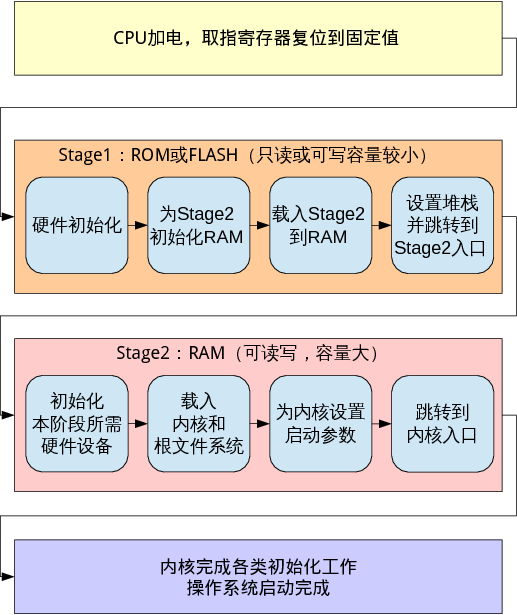
\includegraphics[width=10cm]{bootloader-steps}
  \caption{启动的基本步骤}\label{fig:bootloader-steps} 
\end{figure}

需要注意的是,以上bootloader的两个工作阶段只是从功能上论述内核加载的过程,在具体实现上不同的系统可能有所差别,而且对于不同的硬件环境也会有些不同。
在我们常见的x86 PC的启动过程中,首先执行的是BIOS中的代码,主要完成硬件初始化相关的工作,
然后BIOS会从MBR(master boot record,开机硬盘的第一个扇区)中读取开机信息。在Linux中常说的Grub和Lilo这两种开机管理程序就是保存在MBR中。

\begin{note}
GRUB(GRand Unified Bootloader)是GNU项目的一个多操作系统启动程序。简单的说,就是可以可以用于在有多个操作系统的机器上,
在刚开机的时候选择一个操作系统进行引导。如果安装过Ubuntu一类的发行版的话, 一开机出现的那个选择系统用的菜单就是GRUB提供的。
\end{note}

(这里以Grub为例)BIOS加载MBR中的Grub代码后就把CPU交给了Grub,Grub的工作就是一步一步的加载自身代码,从而识别文件系统,
然后就能够将文件系统中的内核镜像文件加载到内存中,并将CPU控制权转交给操作系统内核。
这样看来,其实BIOS和Grub的前一部分构成了前述stage 1的工作,而stage 2的工作则是完全在Grub中完成的。

\begin{note}
bootloader有两种操作模式:启动加载模式和下载模式。对于普通用户而言,bootloader只运行在启动加载模式,就是我们之前讲解的过程。
而下载模式仅仅对于开发人员有意义,区别是前者是通过本地设备中的内核镜像文件启动操作系统的,而后者是通过串口或以太网等通信手段将远端的内核镜像上载到内存的。
\end{note}

\subsection{gxemul中的启动流程}
从前面的分析,我们可以看到,操作系统的启动是一个非常复杂的过程。不过,幸运的是,由于我们的小操作系统的目标是在gxemul仿真器上运行,
这个过程被大大简化了。gxemul仿真器支持直接加载elf格式的内核,也就是说,gxemul已经提供了bootloader全部功能。
我们的小操作系统不需要再实现bootloader的功能了。换句话说,你可以假定,从我们的小操作系统的运行第一行代码前,
我们就已经拥有一个正常的C环境了。全局变量、函数调用等等C语言运行所需的功能已经可以正常使用了。

\begin{note}
如果你以前对于操作系统的概念仅仅停留在很表面的层次上,那么这里你也许会有所疑惑,为什么我们这里要说“正常的C环境”?
难道还能有“不正常的C环境”?我们来举一个例子说明一下:假定我们刚加电,CPU开始从ROM上取指。
为了简化,我们假定这台机器上没有BIOS(Basic Input Output System),bootloader被直接烧在了ROM中(很多嵌入式环境就是这样做的)。
这时,由于内存没有被初始化,整个bootloader程序尚处于ROM中。程序中的全局变量也仍被储存在ROM上。
而ROM是只读的,所以任何对于全局变量的赋值操作都是不被允许的。可见,此时我们尚不能正常使用C语言的一些特性。
而当内存被初始化,bootloader将后续代码载入到内存中后,位于内存中的代码便能完整地使用C语言的各类功能了。
所以说,内存中的代码拥有了一个正常的C环境。
\end{note}

gxemul支持加载elf格式内核,所以启动流程被简化为加载内核到内存,之后跳转到内核的入口。启动完毕:)整个启动过程非常简单。
这里要注意,之所以简单还有一个原因就在于gxemul本身是仿真器,是一种软件而不是真正的硬件,
所以就不需要面对传统的bootloader面对的那种非常纠结的情况了。

\section{Let's hack the kernel!}

接下来,我们就要开始来折腾我们的小操作系统内核了。这一节中,我们将介绍如何修改内核并实现一些自定义的功能。

\subsection{ssh——远程连接到服务器}
课程提供的整个实验环境位于远程的一台虚拟机上,最终的成果也需要通过这台机器进行提交。因此,我们面临的第一个问题就是:如何操作这台机器?
为了操作这台机器,我们需要通过SSH协议远程连接上它。

一般在Linux或Mac等Unix类环境中都会附带ssh客户端。我们只需要打开终端,然后执行如下指令

\begin{minted}[linenos]{bash}
# username 处填写你的用户名,ip处填写远程主机的地址
$ ssh username@ip
# 之后等候片刻会要求你输入密码,输入的密码不会被显示在屏幕上,输入完成后按回车即可
# 链接后会显示一些欢迎信息,下面是欢迎信息的一个例子
Welcome to Ubuntu 12.04.5 LTS (GNU/Linux 3.13.0-32-generic i686)

 * Documentation:  https://help.ubuntu.com/

  System information as of Tue Aug 11 09:55:40 CST 2015
  System load:  0.0                Processes:           118
  Usage of /:   8.7% of 145.55GB   Users logged in:     0
  Memory usage: 6%                 IP address for eth0: 0.0.0.0
  Swap usage:   0%

  Graph this data and manage this system at:
    https://landscape.canonical.com/

0 packages can be updated.
0 updates are security updates.
# 欢迎信息后会出现命令提示符,等待你输入命令。
\end{minted}

Windows平台下一般不自带ssh,需要下载第三方软件实现这个功能。这里我们使用PuTTY这个小工具实现ssh连接。当然,如果你愿意花时间问问度娘(或Google)的话,
你会发现也有很多功能更为强大ssh客户端软件。不过,鉴于PuTTY小巧简洁且是一个在MIT协议下开源的开源软件,我们这里只介绍PuTTY的用法。

\begin{figure}[htbp]
  \centering
  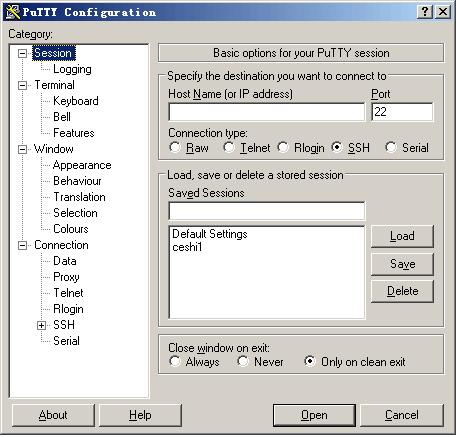
\includegraphics[width=7cm]{putty}
  \caption{PuTTY界面}\label{fig:putty} 
\end{figure}

PuTTY主界面的截图如图\ref{fig:putty}所示。打开PuTTY后,在\textbf{主机名(Host Name)}处填写主机地址(ip),
\textbf{连接方式(Connection type)}处选择\textbf{SSH},\textbf{端口(Port)}使用\textbf{默认值}即可。
之后点击\textbf{连接(Open)}。PuTTY会自动打开一个窗口,按照提示输入用户名和密码即可进入远程主机。

\begin{note}
SSH是Secure Shell的缩写。它是一种用于建立安全的远程连接的网络协议。在Unix类系统上被广泛采用。
除了连接到远程网络,目前SSH还有一种较为有趣的用法。当你既想用Windows,又有时需要Unix环境时,
可以利用Windows8及以上版本自带的Hyper-V开启一个Linux虚拟机(不必开启图形界面)。
之后通过SSH客户端连接到本机上的Linux虚拟机上,即可获得一个Unix环境。甚至可以开启X11转发,
即可在Windows上开启一些Linux上的带图形界面的程序,十分方便。
\end{note}

\subsection{vim 或 nano——阅读并修改代码}
连接到虚拟机以后,我们就可以开始动手阅读并修改代码了。但当你看到光秃秃的命令行的时候,是否感到一阵心慌?
到底该如何打开并编辑一个文件呢?我们先从一个简易的工具入手:nano。

nano的主界面如图\ref{fig:nano}所示。所有基本的操作都被罗列在下面。其中界面上显示的向上的尖状符号(\verb|^|)代表\textbf{Ctrl},
后面的字母就代表相应的快捷键。例如保存是\textbf{Ctrl+O}。nano较为容易上手,但功能相对有限。如果你需要更为强大的功能,可以使用vim。

\begin{figure}[htbp]
  \centering
  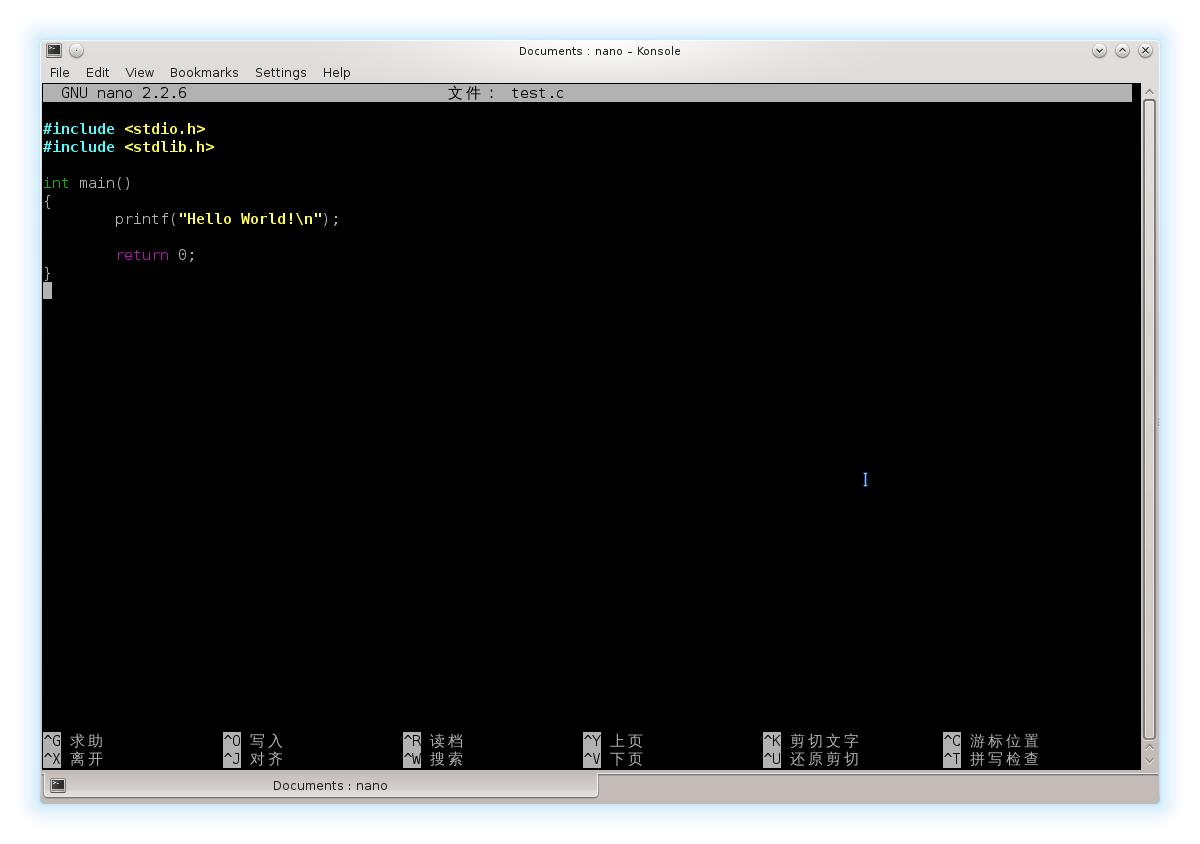
\includegraphics[width=12cm]{nano}
  \caption{nano界面}\label{fig:nano} 
\end{figure}

Vim被誉为编辑器之神,是程序员为程序员设计的编辑器,编辑效率高,十分适合编辑代码。关于如何入门Vim,网络上的资料实在太多,这里就不再赘述了。
推荐一篇质量极高的Vim教程《简明Vim练级攻略》(\url{http://coolshell.cn/articles/5426.html})。只需要十多分钟的阅读,
你就可以掌握Vim的所有基本操作。当然,想要完全掌握它需要相当长的时间去练习。不过,如果你只是想把Vim当成记事本用的话,
那么几分钟的学习足矣。

\subsection{Makefile——内核代码的地图}
当我们学会了Vim,想要翻开代码大干一番的时候,一个新的问题又迎面而来了:这堆代码应当从何读起?答曰:Makefile。当你不知所措的时候,
从Makefile开始往往会是一个不错的选择。这时,有同学又要问了:什么是make?什么又是Makefile呢?
make工具一般用于维护工程。它可以根据时间戳自动判断项目的哪些部分是需要重新编译的,每次只重编译必要的部分。make工具会读取Makefile文件,
并根据Makefile的内容来执行相应的编译操作。Makefile类似于大家以前接触过的VC工程文件。只不过不像VC那样有图形界面,而是直接用类似脚本的方式实现的。

\begin{note}
相较于VC工程而言,Makefile具有更高的\textbf{灵活性}(当然,高灵活性的代价就是学习成本会有所提升,这是必然的),可以方便地管理大型的项目。
而且Makefile理论上支持\textbf{任意的语言},只要其编译器可以通过shell命令来调用。当你的项目可能会混合多种语言,有着复杂的构建流程的时候,
Makefile便能展现出它真正的威力来。
\end{note}

为了使你更为清晰地了解Makefile的基本概念,我们来写一个简单的Makefile。假设我们手头有一个Hello World程序需要编译。我们来为它写一个简易的Makefile。
让我们从头开始,如果我们没有Makefile,直接动手编译这个程序,我们需要下面这样一个指令

\begin{minted}[linenos]{bash}
# 直接使用gcc编译Hello World程序
$ gcc -o hello_world hello_world.c
\end{minted}

那么,如果我们想把它写成Makefile,我们应该怎么办呢?makefile最基本的格式是这样的

\begin{minted}[linenos]{make}
target: dependencies
    command 1
    command 2
    ...
    command n
\end{minted}

其中,target是我们构建(Build)的目标,而dependencies是构建该目标所需的其它文件或其他目标。之后是构建出该目标所需执行的指令。
有一点尤为需要注意:\textbf{每一个指令(command)之前必须有一个TAB}。这里必须使用TAB而不能是空格,否则make会报错。

我们的简易的Makefile可以写成如下的样子,之后执行make即可产生hello\_world这个可执行文件。

\begin{minted}[linenos]{make}
all: hello_world.c
    gcc -o hello_world hello_world.c
\end{minted}

理解了Makefile最基本的概念后,我们来看一下我们的小操作系统的最顶层的Makefile。由于Makefile是用于指导程序如何被构建的,
因此,通过阅读Makefile,我们就可以理解源代码被构建成可执行文件的过程。这一过程可以给我们一些阅读代码的提示,
可以说,Makefile就像源代码的地图,告诉你源代码是如何一步一步成为最终的可执行文件的。代码\ref{code:top-makefile}是实验代码最顶层的Makefile,
通过阅读它我们就能了解代码中很多宏观的东西。

\begin{codeBoxWithCaption}{顶层Makefile\label{code:top-makefile}}
  \inputminted[linenos]{make}{codes/top-Makefile}
\end{codeBoxWithCaption}

如果你以前没有接触过Makefile的话,突然看到这份40行的Makefile可能会有些无奈,完全看不懂啊。不必着急,我们来一行一行地解读它。
前6行是注释,你懂得。7~21行定义了一些变量,包括各个子目录的相对路径,最终的可执行文件的路径(vmlinux\_elf),
linker script的位置(link\_script)。值得注意的两个是modules定义了内核所包含的所有模块,而objects则表示要编译出内核所依赖的所有.o文件。
17到21行行末的斜杠代表这一行没有结束,下一行的内容和这一行是连在一起的。这种写法一般用于提高文件的可读性。可以把本该写在同一行的东西分布在多行中,
使得文件更容易被人类阅读。

\begin{note}
linker script是用于指导连接器将多个.o文件连接成目标可执行文件的脚本。.o文件、linker script等内容我们会在下面的小节中细致地讲解,
大家这里只要知道这些文件是编译内核所必要的就好。
\end{note}

23行的.PHONY表明列在其后的规则不受修改时间的约束。也就是说,一旦该规则被调用,一定保证它被执行。第25行定义all这一规则的依赖。
all代表整个项目,由此我们可以知道,构建整个项目依赖于构建好所有的模块以及vmlinux。那么vmlinux是如何被构建的呢?
紧接着的27行定义了,vmlinux的构建依赖于所有的模块。在构建完所有模块后,将执行第28行的指令来产生vmlinux。
我们可以看到,第28行调用了连接器将之前构建各模块产生的所有.o文件在linker script的指导下连接到一起,产生最终的vmlinux可执行文件。
第30行定义了每个模块的构建方法为调用对应模块目录下的Makefile。最后的33到38行定义了如何清理所有被构建出来的文件。

\begin{note}
一般在写Makefile时,习惯将第一个规则命名为all,也就是构建整个项目的意思。如果调用make时没有指定目标,make会自动执行第一个目标,
所以把all放在第一个目标的位置上,可以使得make命令默认构建整个项目,较为方便。
\end{note}

读到这里,我们会发现还有几个关键的变量没有定义。是的,就是LD、MAKE等出现在编译指令中的变量。紧接着我们看到了第40行有一条include命令。
看来,这个顶层的Makefile还引用了其他的东西。显然这些未定义的变量,是被定义在了这个被include的文件中。被引用的文件如代码\ref{code:include-mk}所示。

\begin{codeBoxWithCaption}{include.mk\label{code:include-mk}}
  \inputminted[linenos]{make}{codes/include.mk}
\end{codeBoxWithCaption}

在该文件中,我们看到了一个非常熟悉的关键词——Cross Compile(交叉编译)。不难看出,这里的CROSS\_COMPILE变量是在定义编译和连接等指令的前缀,
或者说是交叉编译器的具体位置。例如,LD最终调用的指令是“/opt/eldk/usr/bin/mips\_4KC-ld”。通过修改该变量,就可以方便地设定交叉编译工具链的位置。

\begin{exercise}
请修改include.mk文件,使交叉编译器的路径正确。之后执行make指令,如果配置一切正确,则会在gxemul目录下生成vmlinux的内核文件。
\end{exercise}

至此,我们就可以大致掌握阅读Makefile的方法了。善于运用make的功能可以给你带来很多惊喜哦:)提示:可以试着使用一下make clean。
如果你觉得每次用gxemul运行内核都需要打很长的指令这件事很麻烦,那么可以尝试在Makefile中添加运行内核这一功能,使得通过make就能自动运行内核。

\subsection{ELF——深入探究编译与链接}
如果你已经尝试过运行内核,那么你会发现它现在是根本运行不起来的。因为我们还有一些重要的步骤没有做。但是在做这些之前,我们不得不补充一些重要的,
但又有些琐碎的知识。在这里,我们将掀开可执行文件的神秘面纱,进一步去了解一段代码是如何从编译一步一步变成一个可执行文件以及可执行文件又是如何被执行的。

在一切开始之前,请你先泡好一杯茶,慢慢地、耐心地读下去。这一部分的知识对于后面十分重要,但又十分冗长。我们会尽量说得轻松活泼一些,
但由于知识本身的琐碎以及不连贯,所以阅读体验并不会很好。请务必坚持看完:)

\begin{codeBoxWithCaption}{一个简单的C程序\label{code:hello-c}}
  \inputminted[linenos]{c}{codes/hello.c}
\end{codeBoxWithCaption}

我们以代码\ref{code:hello-c}为例,讲述我们这个冗长的故事。我们首先探究这样一个问题:\textbf{含有多个C文件的工程是如何编译成一个可执行文件的?}

这段代码相信你非常熟悉了,不知你有没有注意到过这样一个小细节:printf的定义在哪里?
\footnote{printf位于标准库中,而不在我们的C代码中。将标准库和我们自己编写的C文件编译成一个可执行文件的过程,与将多个C文件编译成一个可执行文件的过程相仿。
因此,我们通过探究printf如何和我们的C文件编译到一起,来展示整个过程。}
我们都学过,C语言中函数必须有定义才能被调用,那么printf的定义在哪里呢?你一定会笑一笑说,别傻了,不就在stdio.h中吗?我们在程序开头通过include引用了它的。
然而事实真的是这样吗?我们来进去看一看stdio.h里到底有些什么。

\begin{codeBoxWithCaption}{stdio.h中关于printf的内容\label{code:part-stdio-h}}
  \inputminted[linenos]{c}{codes/part_of_stdio.h}
\end{codeBoxWithCaption}

在代码\ref{code:part-stdio-h}中,我们展示了从当前系统的stdio.h中摘录出的与printf相关的部分。可以看到,我们所引用的stdio.h中只有声明,但并没有printf的定义。
或者说,并没有printf的具体实现。可没有具体的实现,我们究竟是如何调用printf的呢?我们怎么能够调用一个没有实现的函数呢?

我们来一步一步探究,printf的实现究竟被放在了哪里,又究竟是在何时被插入到我们的程序中的。首先,我们要求编译器\textbf{只进行预处理(通过-E选项)},而不编译。

\begin{minted}[linenos]{c}
/* 由于原输出太长,这里只能留下很少很少的一部分。 */
typedef unsigned char __u_char;
typedef unsigned short int __u_short;
typedef unsigned int __u_int;
typedef unsigned long int __u_long;


typedef signed char __int8_t;
typedef unsigned char __uint8_t;
typedef signed short int __int16_t;
typedef unsigned short int __uint16_t;
typedef signed int __int32_t;
typedef unsigned int __uint32_t;

typedef signed long int __int64_t;
typedef unsigned long int __uint64_t;

extern struct _IO_FILE *stdin;
extern struct _IO_FILE *stdout;
extern struct _IO_FILE *stderr;

extern int printf (const char *__restrict __format, ...);

int main()
{
    printf("Hello World!\n");
    return 0;
}
\end{minted}

可以看到,C语言的预处理器将头文件的内容添加到了源文件中,但同时我们也能看到,这里一阶段并没有printf这一函数的定义。

之后,我们将gcc的-E选项换为-c选项,\textbf{只编译而不链接},产生一个.o目标文件。
我们对其进行反汇编\footnote{为了便于你重现,我们这里没有选择MIPS,而选择了在流行的x86-64体系结构上进行反汇编。
同时,由于x86-64的汇编是CISC汇编,看起来会更为清晰一些。},结果如下

\begin{minted}[linenos]{objdump}
hello.o:     file format elf64-x86-64

Disassembly of section .text:

0000000000000000 <main>:
   0:   55                      push   %rbp
   1:   48 89 e5                mov    %rsp,%rbp
   4:   bf 00 00 00 00          mov    $0x0,%edi
   9:   e8 00 00 00 00          callq  e <main+0xe>
   e:   b8 00 00 00 00          mov    $0x0,%eax
  13:   5d                      pop    %rbp
  14:   c3                      retq
\end{minted}

我们只需要注意中间那句callq即可,这一句是调用函数的指令。对照左侧的机器码,其中e8是call指令的操作码。根据我们在《计算机组成》课程中学习MIPS跳转指令的经验,
e8后面应该跟的是printf的地址。可在这里我们却发现,\textbf{本该填写printf地址的位置上被填写了一串0}。那个地址显然不可能是printf的地址。也就是说,直到这一步,
printf的具体实现依然不在我们的程序中。

最后,我们允许gcc进行连接,也就是\textbf{正常地编译}出可执行文件。然后,再用objdump进行反汇编。

\begin{minted}[linenos]{objdump}
hello:     file format elf64-x86-64


Disassembly of section .init:

00000000004003a8 <_init>:
  4003a8:       48 83 ec 08             sub    $0x8,%rsp
  4003ac:       48 8b 05 0d 05 20 00    mov    0x20050d(%rip),%rax
  4003b3:       48 85 c0                test   %rax,%rax
  4003b6:       74 05                   je     4003bd <_init+0x15>
  4003b8:       e8 43 00 00 00          callq  400400 <__gmon_start__@plt>
  4003bd:       48 83 c4 08             add    $0x8,%rsp
  4003c1:       c3                      retq   

Disassembly of section .plt:

00000000004003d0 <puts@plt-0x10>:
  4003d0:       ff 35 fa 04 20 00       pushq  0x2004fa(%rip)
  4003d6:       ff 25 fc 04 20 00       jmpq   *0x2004fc(%rip)
  4003dc:       0f 1f 40 00             nopl   0x0(%rax)

00000000004003e0 <puts@plt>:
  4003e0:       ff 25 fa 04 20 00       jmpq   *0x2004fa(%rip)
  4003e6:       68 00 00 00 00          pushq  $0x0
  4003eb:       e9 e0 ff ff ff          jmpq   4003d0 <_init+0x28>

00000000004003f0 <__libc_start_main@plt>:
  4003f0:       ff 25 f2 04 20 00       jmpq   *0x2004f2(%rip)
  4003f6:       68 01 00 00 00          pushq  $0x1
  4003fb:       e9 d0 ff ff ff          jmpq   4003d0 <_init+0x28>

0000000000400400 <__gmon_start__@plt>:
  400400:       ff 25 ea 04 20 00       jmpq   *0x2004ea(%rip)
  400406:       68 02 00 00 00          pushq  $0x2
  40040b:       e9 c0 ff ff ff          jmpq   4003d0 <_init+0x28>

Disassembly of section .text:

0000000000400410 <main>:
  400410:       48 83 ec 08             sub    $0x8,%rsp
  400414:       bf a4 05 40 00          mov    $0x4005a4,%edi
  400419:       e8 c2 ff ff ff          callq  4003e0 <puts@plt>
  40041e:       31 c0                   xor    %eax,%eax
  400420:       48 83 c4 08             add    $0x8,%rsp
  400424:       c3                      retq   

0000000000400425 <_start>:
  400425:       31 ed                   xor    %ebp,%ebp
  400427:       49 89 d1                mov    %rdx,%r9
  40042a:       5e                      pop    %rsi
  40042b:       48 89 e2                mov    %rsp,%rdx
  40042e:       48 83 e4 f0             and    $0xfffffffffffffff0,%rsp
  400432:       50                      push   %rax
  400433:       54                      push   %rsp
  400434:       49 c7 c0 90 05 40 00    mov    $0x400590,%r8
  40043b:       48 c7 c1 20 05 40 00    mov    $0x400520,%rcx
  400442:       48 c7 c7 10 04 40 00    mov    $0x400410,%rdi
  400449:       e8 a2 ff ff ff          callq  4003f0 <__libc_start_main@plt>
  40044e:       f4                      hlt    
  40044f:       90                      nop
\end{minted}

篇幅所限,余下的部分没法再展示了(大约还有100来行)。当你看到这段代码的时候,心头一定有一大群草泥马呼啸而过。
什么鬼!我们原本那只可爱的Hello World怎么变成了这副鬼样子!

别急,我们还是只把注意力放在主函数中,这一次,我们可以看到,主函数里那一句callq后面已经不再是一串0了。
那里已经\textbf{被填入了一个地址}。从反汇编代码中我们也可以看到,这个地址就在这个可执行文件里,就在被标记为puts@plt的那个位置上。
虽然高不清楚那货是什么,但显然那就是我们所调用的printf的具体实现了。

由此,我们不难推断,printf的实现是在\textbf{连接(Link)}这一步骤中被插入到最终的可执行文件中的。那么,了解这个细节究竟有什么用呢?
作为一个库函数,printf被大量的程序所使用。因此,每次都将其编译一遍实在太浪费时间了。printf的实现其实早就被编译成了二进制形式。
但此时,printf并未连接到程序中,它的状态与我们利用-c选项产生的hello.o相仿,都还处于未连接的状态。而在编译的最后,
连接器(Linker)会将所有的目标文件连接在一起,将之前未填写的地址等信息填上,形成最终的可执行文件,这就是连接的过程。

对于拥有多个c文件的工程来说,编译器会首先将所有的c文件以文件为单位,编译成.o文件。最后再将所有的.o文件以及函数库连接在一起,
形成最终的可执行文件。整个过程如图\ref{fig:link}所示。

\begin{figure}[htbp]
  \centering
  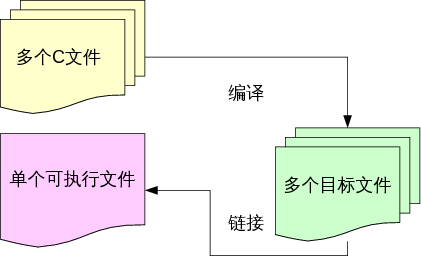
\includegraphics[width=8cm]{link}
  \caption{编译、连接的过程}\label{fig:link} 
\end{figure}

接下来,我们提出我们的下一个问题:\textbf{连接器通过哪些信息来连接多个目标文件呢?}答案就在于在目标文件(也就是我们通过-c选项生成的.o文件)。
在目标文件中,记录了代码各个段的具体信息。连接器通过这些信息来将目标文件链接到一起。而ELF(Executable and Linkable Format)正是Unix上常用的一种目标文件格式。
其实,不仅仅是目标文件,可执行文件也是使用ELF格式记录的。这一点通过ELF的全称也可以看出来。

我们最终生成的内核是ELF格式的,被模拟器载入到内核中。因此,我们暂且只关注ELF是如何被载入到内核中,并且被执行的,
而不再关心具体的连接细节。ELF中有两个相似却不同的概念segment和section。section记录了程序的代码段、数据段等各个段的内容,
主要是连接器在连接的过程中需要使用。而segment则记录了每一段数据(包括代码等内容)需要被载入到哪里,记录了用于指导应用程序加载的各类信息。

我们不妨来看一下,我们之前那个hello world程序的各个segment长什么样子。readelf工具可以方便地解析出elf文件的内容,这里我们使用它来分析我们的程序。

\begin{minted}[linenos]{objdump}
Elf 文件类型为 EXEC (可执行文件)
入口点 0x400e6e
共有 5 个程序头,开始于偏移量64

程序头:
  Type           Offset             VirtAddr           PhysAddr
                 FileSiz            MemSiz              Flags  Align
  LOAD           0x0000000000000000 0x0000000000400000 0x0000000000400000
                 0x00000000000b33c0 0x00000000000b33c0  R E    200000
  LOAD           0x00000000000b4000 0x00000000006b4000 0x00000000006b4000
                 0x0000000000001cd0 0x0000000000003f48  RW     200000
  NOTE           0x0000000000000158 0x0000000000400158 0x0000000000400158
                 0x0000000000000044 0x0000000000000044  R      4
  TLS            0x00000000000b4000 0x00000000006b4000 0x00000000006b4000
                 0x0000000000000020 0x0000000000000050  R      8
  GNU_STACK      0x0000000000000000 0x0000000000000000 0x0000000000000000
                 0x0000000000000000 0x0000000000000000  RW     10

 Section to Segment mapping:
  段节...
   00     .note.ABI-tag .note.gnu.build-id .rela.plt .init .plt .text 
   __libc_freeres_fn __libc_thread_freeres_fn .fini .rodata __libc_subfreeres 
   __libc_atexit __libc_thread_subfreeres .eh_frame .gcc_except_table 
   01     .tdata .init_array .fini_array .jcr .data.rel.ro .got .got.plt .data 
   .bss __libc_freeres_ptrs 
   02     .note.ABI-tag .note.gnu.build-id 
   03     .tdata .tbss 
   04
\end{minted}

这些输出中,我们只需要关注这样几个部分:Offset代表该段(segment)的数据相对于ELF文件的偏移。VirtAddr代表该段最终需要被加载到内存的哪个位置。
FileSiz代表该段的数据在文件中的长度。MemSiz代表该段的数据在内存中所应当占的大小。

\begin{note}
MemSiz永远大于等于FileSiz。若MemSiz大于FileSiz,则操作系统在加载程序的时候,会首先将文件中记录的数据加载到对应的VirtAddr处。
之后,向内存中填0,直到该段在内存中的大小达到MemSiz为止。那么为什么MemSiz有时候会大于FileSiz呢?这里举这样一个例子:
C语言中未初始化的全局变量,我们需要为其分配内存,但它又不需要被初始化成特定数据。因此,在可执行文件中也只记录它需要占用内存(MemSiz),
但在文件中却没有相应的数据(因为它并不需要初始化成特定数据)。故而在这种情况下,MemSiz会大于FileSiz。这也解释了,
为什么C语言中全局变量会有默认值0。这是因为操作系统在加载时将所有未初始化的全局变量所占的内存统一填了0。
\end{note}

VirtAddr是我们尤为需要注意的。由于它的存在,我们就不难推测,Gxemul仿真器在加载我们的内核时,是按照内核这一可执行文件中所记录的地址,
将我们内核中的代码、数据等加载到相应位置。并将CPU的控制权交给内核。我们的内核之所以不能够正常运行,显然是因为我们内核所处的地址是不正确的。
换句话说,\textbf{只要我们能够将内核加载到正确的位置上,我们的内核就应该可以运行起来。}

思考到这里,我们又发现了两个重要的问题。
\begin{enumerate}
  \item 什么叫做正确的位置?到底放在哪里才叫正确。
  \item 哪个段被加载到哪里是记录在编译器编译出来的ELF文件里的,我们怎么才能修改它呢?
\end{enumerate}
在接下来的小节中,我们将一点一点解决掉这两个问题。

\subsection{MIPS内存布局——寻找内核的正确位置}
在这一节中,我们来解决关于内核应该被放在何处的问题。在32位的MIPS CPU中,程序地址空间会被划分为4个大区域。如图\ref{fig:memory-region}所示。

\begin{figure}[htbp]
  \centering
  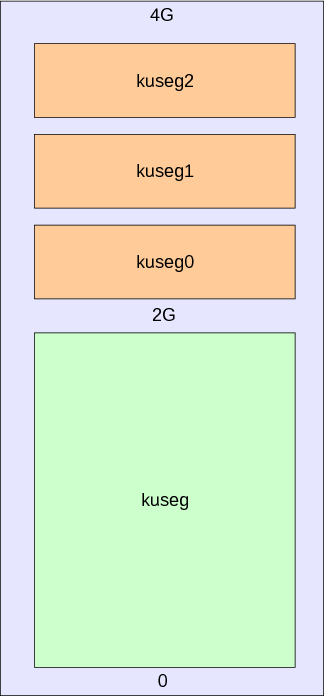
\includegraphics[height=8cm]{memory-region}
  \caption{MIPS内存布局}\label{fig:memory-region} 
\end{figure}

从硬件角度讲,这四个区域的情况如下:

\begin{enumerate}
  \item User Space(kuseg) 0x00000000-0x7FFFFFFF(2G):这些是用户模式下可用的地址。在使用这些地址的时候,程序会通过MMU映射到实际的物理地址上。
  \item Kernel Space Unmapped Cached(kseg0) 0x80000000-0x9FFFFFFF(512MB):只需要将地址的高3 位清零,这些地址就被转换为物理地址。
也就是说,逻辑地址到物理地址的映射关系是硬件直接确的,不通过MMU。因为转换很简单,我们常常把这些地址成为“无需转换的”。
一般情况下,都是通过cache 对这段区域的地址进行访问。
  \item Kernel Space Unmapped Uncached(kseg1) 0xA0000000-0xBFFFFFFF(512MB):这一段地址的转换规则与前者相似,
通过将高3 位清零的方法将地址映射为相应的物理地址,然后映射到物理内存中512MB 大小的低字段。需要注意的是,kseg1 不通过cache 进行存取。
  \item Kernel Space Mapped Cached(kseg2) 0xC0000000-0xFFFFFFFF(1GB):这段地址只能在内核态下使用并且需要MMU 的转换。
\end{enumerate}

看到这里,你也许又蔫儿了,还是完全不知道该把内核放在哪里呀!这里,我们再提供一个提示:需要通过MMU映射访问的地址得在建立虚拟内存机制后才能正常使用,
是由操作系统所管理的。因此,在载入内核时,我们只能选用不需要通过MMU的内存空间,因为此时尚未建立虚存机制。好了,满足这一条件的只有kseg0和kseg1了。
而kseg1是不经过cache的,一般用于访问外部设备。所以,我们的内核只能放在seg0了。

那么具体放在哪里呢?这时,我们就需要仔细阅读代码了。在include/mmu.h里有我们的小操作系统内核完整的内存布局图(代码\ref{code:memory-mmu-h}所示),
在之后的实验中,善用它可以带来意料之外的惊喜。

\begin{codeBoxWithCaption}{include/mmu.h中的内存布局图\label{code:memory-mmu-h}}
  \inputminted[linenos]{c}{codes/memory-mmu.h}
\end{codeBoxWithCaption}

相信聪明的你已经发现了内核的正确位置了吧?

\subsection{Linker Script——控制加载地址}
在发现了内核的正确位置后,我们只需要想办法让内核被加载到那里就OK了。之前在分析ELF文件时我们曾看到过,编译器在生成ELF文件时就已经记录了各段所需要被加载到的位置。
同时,我们也发现,最终的可执行文件实际上是由连接器产生的(它将多个目标文件连接产生最终可执行文件)。因此,我们所需要做的,就是控制连接器的连接过程。

接下来,我们就要引入一个神奇的东西:Linker Script。连接器的设计者们在设计连接器的时候面临这样一个问题:不同平台的ABI(Application Binary Interface)都不一样,
怎样做才能增加连接器的通用性,使得它能为各个不同的平台生成可执行文件呢?于是,就有了Linker Script。Linker Script中记录了各个section应该如何映射到segment,
以及各个segment应该被加载到的位置。下面的指令可以输出默认的连接脚本,你可以在自己的机器上尝试这一条指令:

\begin{minted}[linenos]{bash}
ld --verbose
\end{minted}

这里,我们再补充一下关于ELF文件中section的概念。在链接过程中,目标文件被看成section的集合,并使用section header table来描述各个section的组织。
换句话说,section记录了在连接过程中所需要的必要信息。其中最为重要的三个段为.text、.data、.bss。这三种段的意义是必须要掌握的:

\begin{description}
  \item[.text] 保存可执行文件的操作指令。
  \item[.data] 保存已初始化的全局变量和静态变量。
  \item[.bss] 保存未初始化的全局变量和静态变量。
\end{description}

以上的描述也许会显得比较抽象,这里我们来做一个实验。我们编写一个用于输出代码、全局已初始化变量和全局未初始化变量地址的代码(如代码\ref{code:sections}所示)。
观察其运行结果与ELF文件中记录的.text、.data和.bss段相关信息之间的关系。

\begin{codeBoxWithCaption}{用于输出各section地址的程序\label{code:sections}}
  \inputminted[linenos]{c}{codes/sections.c}
\end{codeBoxWithCaption}

该程序的一个可能的输出如下\footnote{在不同机器上运行,结果也许会有一定的差异}。

\begin{minted}[linenos]{bash}
user@debian ~/Desktop $ ./program 
80D4188
80D60A0
8048AAC
\end{minted}

我们再看看ELF文件中记录的各section的相关信息(为了突出重点,这里只保留我们所关心的section)。

\begin{minted}[linenos]{objdump}
共有 29 个节头,从偏移量 0x9c258 开始:

节头:
  [Nr] Name              Type            Addr     Off    Size   ES Flg Lk Inf Al
  [ 4] .text             PROGBITS        08048140 000140 0620e4 00  AX  0   0 16
  [22] .data             PROGBITS        080d4180 08b180 000f20 00  WA  0   0 32
  [23] .bss              NOBITS          080d50c0 08c0a0 00136c 00  WA  0   0 64
\end{minted}

对比二者,我们就可以清晰的知道,\textbf{.text段包含了可执行文件中的代码},\textbf{.data段包含了需要被初始化的全局变量和静态变量},
而\textbf{.bss段包含了无需初始化的全局变量和静态变量}

接下来,我们通过Linker Script来尝试调整各段的位置。这里,我们选用GNU LD官方帮助文档上的例子
(\url{https://www.sourceware.org/binutils/docs/ld/Simple-Example.html#Simple-Example})
该例子的完整代码如下所示:

\begin{minted}[linenos]{objdump}
SECTIONS
{
   . = 0x10000;
   .text : { *(.text) }
   . = 0x8000000;
   .data : { *(.data) }
   .bss : { *(.bss) }
}
\end{minted}

在第三行的“.”是一个特殊符号,用来做定位计数器,它根据输出段的大小增长。在SECTIONS命令开始的时候,它的值为0。通过设置“.”即可设置接下来的section的其实地址。
“*”是一个通配符,匹配所有的相应的段。例如“.bss:\{*(.bss)\}”表示将所有输入文件中的.bss段(右边的.bss)都放到输出的.bss段(左边的.bss)中。
为了能够编译通过(这个脚本过于简单,难以用于连接真正的程序),我们将原来的实验代码简化如下

\begin{minted}[linenos]{c}
char msg[]="Hello World!\n";
int count;

int main()
{
    return 0;
}
\end{minted}

编译,并查看生产的可执行文件各section的信息。

\begin{minted}[linenos]{objdump}
user@debian ~/Desktop $ gcc -o test test.c -T test.lds -nostdlib -m32
user@debian ~/Desktop $ readelf -S test                              
共有 11 个节头,从偏移量 0x2164 开始:

节头:
  [Nr] Name              Type            Addr     Off    Size   ES Flg Lk Inf Al
  [ 2] .text             PROGBITS        00010024 001024 00000a 00  AX  0   0  1
  [ 5] .data             PROGBITS        08000000 002000 00000e 00  WA  0   0  1
  [ 6] .bss              NOBITS          08000010 00200e 000004 00  WA  0   0  4
\end{minted}

可以看到,在使用了我们自定义的Linker Script以后,生成的程序各个section的位置就被调整到了我们所指定的地址上。
segment是由section组合而成的,section的地址被调整了,那么最终segment的地址也会相应地被调整。
至此,我们就了解了如何通过lds文件控制各段被加载到的位置。

\begin{exercise}
填写tools/scse0\_3.lds中空缺的部分,将内核调整到正确的位置上。
\end{exercise}

再补充一点:关于链接后的程序从何处开始执行。程序执行的第一条指令称为entry point,
我们在linker script中可以通过ENTRY(function name)指令来设置程序入口。linker中程序入口的设置方法有以下五种:
\begin{enumerate}
  \item 使用ld命令时,通过参数“-e”设置
  \item 在linker scirpt中使用ENTRY()指令指定了程序入口
  \item 如果定义start,则start就是程序入口
  \item .text段的第一个字节
  \item 地址0处
\end{enumerate}
在我们的实验中,采用了其中的第二种方式指定了程序入口。

\section{MIPS汇编与C语言}
在这一节中,我们将简单介绍MIPS汇编,以及常见的C语言语法与汇编的对应关系。在操作系统编程中,不可避免地要接触到汇编语言。
我们经常需要从C语言中调用一些汇编语言写成的函数,或者反过来,在汇编中跳转到C函数。为了能够实现这些,
我们需要了解C语言与汇编之间千丝万缕的联系。

我们代码\ref{code:c-example}为例,介绍典型的C语言中的语句对应的汇编代码。

\begin{codeBoxWithCaption}{样例程序\label{code:c-example}}
  \inputminted[linenos]{c}{codes/example.c}
\end{codeBoxWithCaption}

\subsection{循环与判断}
这里你可能会问了,样例代码里只有循环啊!哪里有什么判断语句呀?事实上,由于MIPS汇编中没有循环这样的高级结构,
所有的循环均是采用判断加跳转语句实现的,所以我们将循环语句和判断语句合并在一起进行分析。
我们分析代码的第一步,就是要将循环等高级结构,用\textbf{判断加跳转}的方式替代。
例如,代码\ref{code:c-example}第13-15行的循环语句,其最终的实现可能就如下面的C代码所展示的那样。

\begin{minted}[linenos]{c}
      i = 0;
      goto CHECK;
FOR:  sum += fib(i);
      ++i;
CHECK:if (i < 10) goto FOR;
\end{minted}

将样例程序编译\footnote{为了生成更简单的汇编代码,我们采用了-nostdlib -static -mno-abicalls这三个编译参数},
我们观察其反汇编代码。对照汇编代码和我们刚才所分析出来的C代码。
我们基本就能够看出来其间的对应关系。这里,我们将对应的C代码标记在反汇编代码右侧。

\begin{minted}[linenos]{objdump}
  400158:       sw      zero,16(s8)           #       sum = 0;
  40015c:       sw      zero,20(s8)           #       i = 0;
  400160:       j       400190 <main+0x48>    #       goto CHECK;
  400164:       nop                           # --------------------
  400168:       lw      a0,20(s8)             #  FOR:
  40016c:       jal     4000b0 <fib>          #
  400170:       nop                           #
  400174:       move    v1,v0                 #        sum += fib(i);
  400178:       lw      v0,16(s8)             #
  40017c:       addu    v0,v0,v1              #
  400180:       sw      v0,16(s8)             #
  400184:       lw      v0,20(s8)             # --------------------
  400188:       addiu   v0,v0,1               #        ++i;
  40018c:       sw      v0,20(s8)             # --------------------
  400190:       lw      v0,20(s8)             # CHECK:
  400194:       slti    v0,v0,10              #        if (i < 10)
  400198:       bnez    v0,400168 <main+0x20> #            goto FOR;
  40019c:       nop
\end{minted}

再将右边的C代码对应会原来的C代码,我们就能够大致知道每一条汇编语句所对应的原始的C代码是什么了。
可以看出,判断和循环主要采用slt、slti判断两数间的大小关系,再结合b类型指令根据对应条件跳转。
以这些指令为突破口,我们就能大致识别出循环结构、分支结构了。

\subsection{函数调用}
这里需要区分函数的调用方和被调用方来分别分析。我们选用样例程序中的fib这个函数来观察函数调用相关的内容。
这个函数是一个递归函数,因此,它函数调用过程的调用者,同时也是被调用者。我们可以从中观察到如何调用一个函数,
以及一个被调用的函数应当做些什么工作。

我们还是先将整个函数调用过程用高级语言来表示一下。
\begin{minted}[linenos]{c}
int fib(int n)
{
        if (n == 0) goto BRANCH;
        if (n != 1) goto BRANCH2;
BRANCH: v0 = 1;
        goto RETURN;
BRANCH2:v0 = fib(n-1) + fib(n-2);
RETURN: return v0;
}
\end{minted}

然而,之后在分析汇编代码的时候,我们会发现有很多C语言中没有表示出来的东西。例如,在函数开头,有一大串的sw,
结尾处又有一大串的lw。这些东西究竟是在做些什么呢?

\begin{minted}[linenos]{objdump}
004000b0 <fib>:
  4000b0:       27bdffd8        addiu   sp,sp,-40
  4000b4:       afbf0020        sw      ra,32(sp)
  4000b8:       afbe001c        sw      s8,28(sp)
  4000bc:       afb00018        sw      s0,24(sp)
  # 中间暂且掠过,只关注一系列sw和lw操作。
  400130:       8fbf0020        lw      ra,32(sp)
  400134:       8fbe001c        lw      s8,28(sp)
  400138:       8fb00018        lw      s0,24(sp)
  40013c:       27bd0028        addiu   sp,sp,40
  400140:       03e00008        jr      ra
  400144:       00000000        nop
\end{minted}

我们来回忆一下C语言的递归。在经过了《数据结构》这门课程的学习后,你一定发现了,递归的过程和栈这种数据结构有着惊人的相似性。
每一次递归操作就仿佛将当前函数的所有变量和状态压入了一个栈中,待到返回时再从栈中弹出来。

好了,回忆起了这个细节,我们再来看看汇编代码。在函数的开头,编译器为我们添加了一组sw操作,
将所有当前函数所需要用到的寄存器原有的值全部保存到了内存中
\footnote{其实这样说并不准确,后面我们会看到,有些寄存器的值是由调用者负责保存的,有些是由被调用者保存的。但这里为了理解方便,
我们姑且认为被调用的函数保存了调用者的所有状态吧}。而在函数返回之前,编译器又加入了一组lw操作,将值被改变的寄存器全部恢复为原有的值。

我们惊奇地发现:编译器在函数调用的前后为我们添加了一组压栈(push)和弹栈(pop)的操作,为我们保存了函数的当前状态。
函数的开始,编译器首先\textbf{减小sp指针的值,为栈分配空间}。并将需要保存的值放置在栈中。
当函数将要返回时,编译器再\textbf{增加sp指针的值,释放栈空间}。同时,恢复之前被保存的寄存器原有的值。
这就是为何C语言的函数调用和栈有着很大的相似性的原因:在函数调用过程中,编译器真的为我们维护了一个栈。

\begin{note}
ra寄存器存放了函数的返回地址。使得被调用的函数结束时得以返回到调用者调用它的地方。但你有没有想过,我们其实可以将这个返回点设置为别的函数的入口,
使得该函数在返回时直接进入另一个函数中,而不是回到调用者哪里?一个函数调用了另一个函数,而返回时,返回到第三个函数中,
是不是也是一种很有价值的编程模型呢?如果你对此感兴趣,可以了解一下函数式编程中的Continuations的概念
(推荐\href{https://github.com/justinyhuang/Functional-Programming-For-The-Rest-of-Us-Cn/blob/master/FunctionalProgrammingForTheRestOfUs.cn.md}
{Functional Programming For The Rest Of Us}这篇文章),
在很多新近流行起来的语言中,都引入了类似的想法。
\end{note}

在我们看到了一个函数作为被调用者做了哪些工作后,我们再来看看,作为函数的调用者需要做些什么?如何调用一个函数?如何传递参数?又如何获取返回值?
让我们来看一下,fib函数调用fib(n-1)和fib(n-2)时,编译器为我们生成的汇编代码\footnote{为了方便你了解自己手写汇编时应当怎样写,我们这一次采用汇编代码,
而不是反汇编代码。这里注意,fp和上面反汇编出的s8其实是同一个寄存器,只是有两个不同的名字而已}

\begin{minted}[linenos]{gas}
lw      $2,40($fp)      # v0 = n;
addiu   $2,$2,-1        # v0 = a0 - 1;
move    $4,$2           # a0 = v0;      // 即a0=n-1
jal     fib             # v0 = fib(a0);
nop                     #

move    $16,$2          # s0 = v0;
lw      $2,40($fp)      # v0 = n;
addiu   $2,$2,-2        # v0 = n - 2;
move    $4,$2           # a0 = v0;      // 即a0=n-2
jal     fib             # v0 = fib(a0);
nop                     #

addu    $16,$16,$2      # s0 += v0;
sw      $16,16($fp)     #
\end{minted}

我们将汇编所对应的语义用C语言标明在右侧。可以看到,调用一个函数就是将参数存放在a0-a3寄存器中(我们暂且不关心参数非常多的函数会处理),
然后使用jal指令跳转到相应的函数中。函数的返回值会被保存在v0-v1寄存器中。我们通过这两个寄存器的值来获取返回值。

\begin{exercise}
完成boot/start.S中空缺的部分。设置栈指针,跳转到main函数。
使用gxemul –E testmips –C R3000 –M 64 elf-file运行(其中elf-file是你编译生成的vmlinux文件的路径)。 
\end{exercise}

在调用main函数之前,我们需要将sp寄存器设置到内核栈空间的位置上。具体的地址可以从mmu.h中看到。
这里做一个提醒,请注意栈的增长方向。设置完栈指针后,我们就具备了执行C语言代码的条件,因此,
接下来的工作就可以交给C代码来完成了。所以,在start.S的最后,我们调用C代码的主函数,
正式进入内核的C语言部分。

\subsection{通用寄存器使用约定}
为了和编译器等程序相互配合,我们需要遵循一些使用约定。这些规定与硬件无关,硬件并不关心寄存器具体被用于什么用途。
这些规定是为了让不同的软件之间得以协同工作而制定的。MIPS中一共有32个通用寄存器(General Purpose Registers),
其用途如表\ref{tab:registers}所示。

\begin{table}[h]
  \centering
  \begin{tabular}{ccp{10cm}}
    \toprule
    寄存器编号 & 助记符 & 用途 \\
    \midrule
    0   & zero & 值总是为0\\
    1   & at   & (汇编暂存寄存器)一般由汇编器作为临时寄存器使用。\\
    2-3 & v0-v1& 用于存放表达式的值或函数的整形、指针类型返回值\\
    4-7 & a0-a3& 用于函数传参。其值在函数调用的过程中不会被保存。若函数参数较多,多出来的参数会采用栈进行传递\\
    8-15& t0-t7& 用于存放表达式的值的临时寄存器;其值在函数调用的过程中不会被保存。\\
    16-23&s0-s7& 保存寄存器;这些寄存器中的值在经过函数调用后不会被改变。\\
    24-25&t8-t9& 用于存放表达式的值的临时寄存器;其值在函数调用的过程中不会被保存。当调用位置无关函数(position independent function)时,
               25号寄存器必须存放被调用函数的地址。\\
    26-27&kt0-kt1& 仅被操作系统使用。\\
    28  & gp   & 全局指针和内容指针。\\
    29  & sp   & 栈指针。\\
    30  &fp或s8& 保存寄存器(同s0-s7)。也可用作帧指针。\\
    31  & ra   & 函数返回地址。\\
    \bottomrule
  \end{tabular}
  \caption{MIPS通用寄存器\label{tab:registers}}
\end{table}

其中,只有16-23号寄存器和28-30号寄存器的值在函数调用的前后是不变的\footnote{请注意,这里的不变并不意味着它们的值在函数调用的过程中不能被改变。
只是指它们的值在函数调用后和函数调用前是一致的。}。
对于28号寄存器有一个特例:当调用位置无关代码(position independent code)时,28号寄存器的值是不被保存的。

除了这些通用寄存器之外,还有一个特殊的寄存器:PC寄存器。这个寄存器中储存了当前要执行的指令的地址。
当你在Gxemul仿真器上调试内核时,可以留意一下这个寄存器。通过PC的值,我们就能够知道当前内核在执行的代码是哪一条,
或者触发中断的代码是哪一条等等。

\section{实战printf}
了解了这么多的内容后,我们来进行一番实战,在内核中实现一个printf函数。
在平时使用中,你可能觉得printf函数是由语言本身提供的,其实不是,printf全都是由C语言的标准库提供的。
而C语言的标准库是建立在操作系统基础之上的。所以,当我们开发操作系统的时候,我们就会发现,我们失去了C语言标准库的支持。
我们需要用到的几乎所有东西,都需要我们自己来实现。

要弄懂系统如何将一个字符输出到终端当中,需要阅读以下三个文件:lib/printf.c,lib/print.c和drivers/gxconsole/console.c。
相信阅读这些代码对于聪明的你来说,完全不是问题,我们就不再赘述了。

\begin{exercise}
阅读相关代码,并补全lib/print.c中lp\_Print()函数中缺失的部分来实现字符输出。
\end{exercise}

当你刚看到lp\_Print()的代码时,也许会手忙脚乱。不知如何读起,更不清楚该如何补全它。这主要是由于,我们对于printf要实现的具体功能没有完整的认识。
这里我们给出一些提示,printf的format specifier(也就是它的第一个参数)的格式如下:

\begin{equation*}
  \%[flags][width][.precision][length]specifier 
\end{equation*}

更详尽的描述,请大家查询C语言标准库的相关文档\footnote{推荐cplusplus,这个网站给出了很多的样例
\url{http://www.cplusplus.com/reference/cstdio/printf/}}。完整的描述较为复杂,我们只需实现我们所有能够支持的部分即可。
例如,内核中是无法使用浮点数的,因此所有和浮点输出相关的东西都不必要实现。

\section{实验正确结果}
如果你正确地实现了前面所要求的全部内容,你将在gxemul中观察到如下输出,这标志着你顺利完成了lab1实验(仍需阅读本章中余下的内容,以便掌握提交代码所需的git技能)。

\begin{minted}[linenos]{text}
GXemul 0.4.6    Copyright (C) 2003-2007  Anders Gavare
Read the source code and/or documentation for other Copyright messages.

Simple setup...
    net: simulating 10.0.0.0/8 (max outgoing: TCP=100, UDP=100)
        simulated gateway: 10.0.0.254 (60:50:40:30:20:10)
            using nameserver 202.112.128.51
    machine "default":
        memory: 64 MB
        cpu0: R3000 (I+D = 4+4 KB)
        machine: MIPS test machine
        loading gxemul/vmlinux
        starting cpu0 at 0x80010000
-------------------------------------------------------------------------------

main.c:	main is start ...

init.c:	mips_init() is called

panic at init.c:24: ^^^^^^^^^^^^^^^^^^^^^^^^^^^^^^^^^^^^^
\end{minted}

\section{Git——轻松维护和提交代码}

在完成了这次实验后,你刚刚伸了个懒腰。突然,一个问题浮现在了你的脑海中:如何提交刚刚完成的实验代码呢?
整个实验的代码采用了git版本控制系统进行管理,所有与代码管理相关的操作全部通过git完成。
在本章最后的部分,我们就来了解一下git相关的内容。

\subsection{手工的版本控制}

最原始的版本控制是纯手工的版本控制:修改文件,保存文件副本。有时候偷懒省事,保存副本时命名比较随意,时间长了就不知道哪个是新的,哪个是老的了,即使知道新旧,可能也不知道每个版本是什么内容,相对上一版作了什么修改了,当几个版本过去后,很可能就是下面的样子了:

\begin{figure}[htbp]
  \centering
  \includegraphics[width=5cm]{git-example}
  \caption{手工版本控制效果图}\label{fig:git-example}
\end{figure}

当然,有些时候,我们不仅是一个人写论文,很可能是多个人同时写一篇paper。

分工,制定计划,埋头苦干,看起来一切都井然有序,后来却只会让人蛋疼不已。本质原因在于每个人都会对书的内容进行改动,结果最后成了这样的情形:我把我修订的最新版的电子版发邮件给他,然后,我继续修改书的内容。一天后,他再把电子书传给我。每到此时,我就必须想清楚,发给他之后到我收到他的文件期间,我在哪里作了哪些改动,还得把我的改动和他的部分合并,真困难。

到这时我们发现一个无法避免的事实:如果每一次小小的改动都要通知对方,那么一些错误的改动将会令我们付出很大的代价:一个错误的改动要频繁在两方同时通知纠正。但如果一次性改动大幅度的内容,尤其是在不连续的段落中删删改改,将变成只有阅读完整篇论文才能知道对方在哪里改动过,才能把两个人的劳动成果合并。论文只有10页时还可以接受,但如果变成20页,50页,100页呢?

后来我们就想如果能有这样一个软件:
\begin{itemize}
\item 自动帮我记录每次文件的改动,而且最好是有后悔药的功能,改错了一个东西,我可以轻松撤销。
\item 还得有多人协作编辑不费力的好处,有着简洁的指令与操作。
\item 最好能像时光机一样穿越回以前,而且不但能穿越回去,还能在不满意的时候穿越回来!
\item 如果想查看某次改动,只需要在软件里瞄一眼就可以。
\end{itemize}

那岂不是十分方便!

版本控制系统就是这样一种神奇的系统。而git,则是目前世界上最先进的分布式版本控制系统,没有之一。
\begin{note}
版本控制是一种记录若干文件内容变化,以便将来查阅特定版本修订情况的系统。
\end{note}

\subsection{Git基础指引}
看过那个小故事后,相信大家对git这个世界上目前最先进的分布式版本控制系统已经产生了很强的兴趣。简单地说,Git 究竟是怎样的一个系统呢?别着急,我们慢慢来。

先从git的最基础的指令讲起

\begin{minted}[linenos]{bash}
$ git init
\end{minted}

使用命令
\begin{minted}[linenos]{bash}
$ sudo mkdir learnGit
\end{minted}
使用 cd learnGit 进入后,执行 git init 创建新的 git 仓库。这时候细心的同学会发现在我们的新文件夹下其实已经有东西了,我们可以使用
\begin{minted}[linenos]{bash}
$ ls -a
\end{minted}
来观察,我们看到我们的文件夹下多出一个名叫 .git 的目录,这个隐藏的 .git 目录就是 Git 版本库,更多时候我们称之为仓库(repository)。仓库是用于跟踪管理版本库的,\textbf{在我们的实验中不会对 .git 文件夹下的文件进行任何操作,所以不要对该文件夹中的任何文件进行任何手工修改}!

在刚刚我们提到的\textbf{init} 命令完成之后,我们就已经有了一个仓库。我们之前所建立的 learnGit 这个文件夹就是Git 里的 工作区。目前我们的工作区除了包含一个隐藏的 .git 版本库目录外空无一物。

\begin{note}
在我们的小操作系统实验中我们不需要使用到 git init 命令,每个人一开始就都有一个名为 1406xxxx-lab 的版本库,包含了lab1的实验内容。
\end{note}

我们的工作区现在空荡荡的,我们来为它加点料。我们使用下面的指令创建一个新的文本文件
\begin{minted}[linenos]{bash}
$ echo "BUAA_OSLAB" > readme.txt
\end{minted}

这一步只是创建一个文本文件而已,为了将它添加到版本库,我们需要执行下面的命令

\begin{minted}[linenos]{bash}
$ git add readme.txt
\end{minted}
\label{git add}
注意,到这里还没有结束,你可能会想,那我既然都把 readme.txt 加入了,难道不是已经提交到版本库了吗?但事实就是这样,Git——同其他大多数版本控制系统一样,add 之后需要再执行一次提交操作,提交操作的命令如下

\begin{minted}[linenos]{bash}
$ git commit
\end{minted}

如果不带任何附加选项的话,git commit 后会弹出一个说明窗口,如下所示

\begin{minted}[linenos]{bash}
GNU nano 2.2.6    文件: /home/13061193/13061193-lab/.git/COMMIT_EDITMSG              

Notes to test.
# 请为您的变更输入提交说明。以 '#' 开始的行将被忽略,而一个空的提交
# 说明将会终止提交。
# 位于分支 master
# 您的分支与上游分支 'origin/master' 一致。
#
# 要提交的变更:
#       修改:         readme.txt
#

                                 [ 已读取9 行 ]
^G 求助      ^O 写入      ^R 读档      ^Y 上页      ^K 剪切文字  ^C 游标位置
^X 离开      ^J 对齐      ^W 搜索      ^V 下页      ^U 还原剪切  ^T 拼写检查
\end{minted}


在上面里书写的 \textbf{Notes to test.}是我们本次提交所附加的说明。
注意,弹出的窗口中我们\textbf{必须}得添加本次commit的说明,这意味着我们不能提交空白说明,否则我们的提交不会成功。而且在添加评论之后,可以按提示按键来成功保存。

\begin{note}
初学者一般不太重视git commit内容的有效性,总是使用无意义的字符串作为说明提交。但以后你可能就会发现自己写了一个自己看得懂,别人也能看得懂提交说明是多么庆幸。所以尽量让你的每次提交显得有意义,比如“fixed a bug in ..."这样的描述,顺便推荐一条命令:git commit -{}-amend,这条命令可以重新书写你最后一次commit的说明。
\end{note}

这样窗口提交的方式比较繁琐,我们可以采取一种较为简洁的方式\label{git commit}
\begin{minted}[linenos]{bash}
$ git commit -m [comments]
\end{minted}

[comments]格式为\textbf{“评论内容”},上述的提交过程我们可以简化为下面一条指令

\begin{minted}[linenos]{bash}
$ git commit -m "Notes to test."
\end{minted}

如果我们在提交后看到类似提示就说明我们提交成功了

\begin{minted}[linenos]{bash}
[master 955db52] Notes to test.
 1 file changed, 1 insertion(+), 1 deletion(-)
\end{minted}
从我们本次提交中我们可以得到以下信息,可能现在你还不能完全理解这些信息代表的意思,但是没关系,之后我们会讲解

\begin{itemize}
\item 本次提交的分支\label{分支}是 master
\item 本次提交的ID是 955db52
\item 提交说明是 Notes to test
\item 共有1个文件相比之前发生了变化:1行的添加与1行的删除行为
\end{itemize}

但是在我们实验中,第一次提交可不会这么一帆风顺,我们第一次提交往往会出现下面的提示

\begin{minted}[linenos]{c}
*** Please tell me who you are.

Run

  git config --global user.email "you@example.com"
  git config --global user.name "Your Name"

# to set your account’s default identity.
# Omit --global to set the identity only in this repository.
\end{minted}

相信大家从第一句也能推测出,这是要求我们设置提交者身份的。我们设置身份有什么作用呢?别急,等你设置成功了我们再详谈。

\begin{note}
从上面我们也知道了,我们可以用  

  git config -{}-global user.email “you@example.com”
  
  git config -{}-global user.name “Your Name“
  
这两条命令设置我们的名字和邮箱,在我们的实验中对这两个没有什么要求,大家随性设置就好,给个示例:

  git config -{}-global user.email “qianlxc@126.com”
  
  git config -{}-global user.name “Qian”
\end{note}

现在你已设置了提交者的信息,那么做一下这个小练习来快速上手Git的使用吧

\begin{exercise}
	\begin{itemize}
		\item 在/home/1406xxxx/ 目录下创建一个名为 README.txt的文件。这时使用 git status > Untracked.txt 。
		\item 在README.txt文件中随便写点什么,然后使用刚刚学到的 add 命令,再使用 git status > Stage.txt 。
		\item 之后使用上面学到的 Git 提交有关的知识把README.txt提交,并在提交说明里写入自己的学号。
		\item 使用 cat Untracked.txt 和 cat Stage.txt,对比一下两次的结果,体会一下README.txt 两次所处位置的不同。
		\item 修改 README.txt 文件,再使用 git status > Modified.txt 。
		\item 使用 cat Modified.txt ,观察它和第一次 add 之前的 status 一样吗,思考一下为什么?
	\end{itemize}
\end{exercise}

\begin{note}
git status 是一个查看当前文件状态的有效指令,而git log则是提交日志,每commit 一次,Git会在提交日志中记录一次。git log将在我们后面乘坐时光机时发挥很大的作用。
\end{note}

相信你做过上述实验后,心里还是会有些疑惑,没关系,我们来一起看一下我们刚才得到的 Untracked.txt , Stage.txt 和 Modified.txt 的内容

\begin{minted}[linenos]{bash}
Untracked.txt的内容如下

# On branch master
# Untracked files:
#   (use "git add <file>..." to include in what will be committed)
#
#	README.txt
nothing added to commit but untracked files present (use "git add" to track)

Stage.txt的内容如下

# On branch master
# Changes to be committed:
#   (use "git reset HEAD <file>..." to unstage)
#
#	new file:   README.txt
#

Modified.txt的内容如下

# On branch master
# Changes not staged for commit:
#   (use "git add <file>..." to update what will be committed)
#   (use "git checkout -- <file>..." to discard changes in working directory)
#
#	modified:   README.txt
#
no changes added to commit (use "git add" and/or "git commit -a")
\end{minted}

通过仔细观察,我们看到第一个文本文件中第2行是:Untraced files,而第二个文本文件中第二行内容是:Changes to be committed,而第三个则是Changes not staged for commit。这三种不同的提示意味着什么,需要你通过后面的学习找到答案,答案就在不远处。

我们开始时已经介绍了Git中的工作区的概念,接下来的内容就是 Git 中的最核心的概念,为了能自如运用Git 中的命令,你一定要仔细学习。

\subsection{Git文件四状态}
首先对于任何一个文件,在 Git 内都只有四种状态:未跟踪(untracked)、未修改(unmodified)、已修改(modified)、已暂存(staged)
\begin{description}
\item[未跟踪] 表示没有跟踪(add)某个文件的变化,使用git add即可跟踪文件
\item[未修改] 表示某文件在跟踪后一直没有改动过或者改动已经被提交
\item[已修改] 表示修改了某个文件,但还没有加入(add)到暂存区中
\item[已暂存] 表示把已修改的文件放在下次提交(commit)时要保存的清单中
\end{description}

\begin{note}
关于刚才的exercise中的思考,实际上是因为git add 指令本身是有多义性的,虽然差别较小但是不同情境下使用依然是有区别。我们现在只需要记住:新建文件后要git add,修改文件后也需要git add。
\end{note}

我们使用一张图来说明文件的四种状态的转换关系

\begin{figure}[htbp]
	\centering
	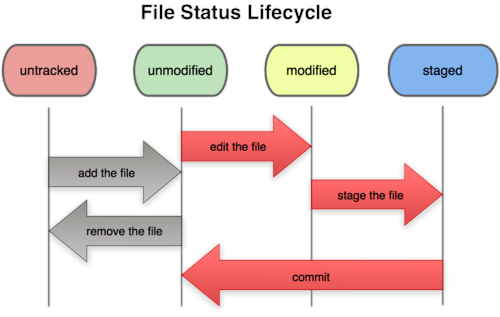
\includegraphics[width=9.5cm]{git-change}
	\caption{Git中的四种状态转换关系}\label{fig:git-change}
\end{figure}

\begin{exercise}
仔细看看这张图,思考一下红箭头里的 add the file 、 stage the file 和 commit 分别对应的是Git里的哪些命令呢?
\end{exercise}

看到这里,相信你对Git的设计有了初步的认识。下一步我们就来深入理解一下Git里的一些机制,从而让我们可以一次上手,终身难忘。

\subsection{Git三棵树}\label{Git三棵树}
我们的本地仓库由 git 维护的三棵“树”组成。第一个是我们的工作区,它持有实际文件;第二个是 暂存区(Index有时也称Stage),它像个暂时存放的区域,临时保存你的改动;最后是HEAD,指向你最近一次提交后的结果。

在我们的.git 目录中,文件 .git/index 实际上就是一个包含文件索引的目录树,像是一个虚拟的工作区。在这个虚拟工作区的目录树中,记录了文件名、文件的状态信息(时间戳、文件长度等),但是\textbf{文件的内容并不存储其中,而是保存在 Git 对象库(.git/objects)中},文件索引建立了文件和对象库中对象实体之间的对应。下面这个图展示了工作区、版本库中的暂存区和版本库之间的关系\footnote{这张图转载自网站\url{http://www.worldhello.net/2010/11/30/2166.html}},希望你能耐着性子仔细理解这张图和不同操作所带来的不同影响。

\begin{figure}[htbp]
  \centering
  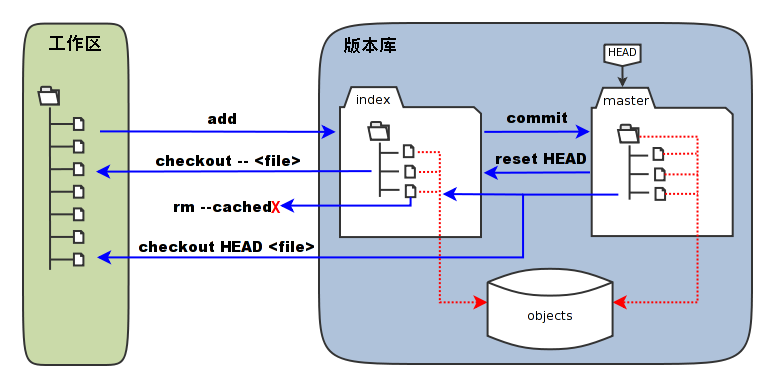
\includegraphics[width=15cm]{git-stage}
  \caption{工作区、暂存区和版本库}\label{fig:git-stage} 
\end{figure}

\begin{itemize}
\item 图中 objects 标识的区域为 Git 的对象库,实际位于 ".git/objects" 目录下。
\item 图中左侧为工作区,右侧为版本库。在版本库中标记为 "index" 的区域是暂存区(stage, index),标记为 "master" 的是 master 分支所代表的目录树。
\item 图中我们可以看出此时 "HEAD" 实际是指向 master 分支的一个“游标”。所以图示的命令中出现 HEAD 的地方可以用 master 来替换。
\item 当对工作区修改(或新增)的文件执行 "git add" 命令时,暂存区的目录树被更新,同时工作区修改(或新增)的文件内容被写入到对象库中的一个新的对象中,而该对象的ID 被记录在暂存区的文件索引中。
\item 当执行提交操作(git commit)时,会将暂存区的目录树写到版本库(对象库)中,master 分支会做相应的更新。即 master 指向的目录树就是提交时暂存区的目录树。
\item 当执行 "git rm -{}-cached <file>" 命令时,会直接从暂存区删除文件,工作区则不做出改变。
\item 当执行 "git reset HEAD" 命令时,暂存区的目录树会被重写,被 master 分支指向的目录树所替换,但是工作区不受影响。
\item 当执行 "git checkout -{}- <file>" 命令时,会用暂存区指定的文件替换工作区的文件。这个操作很危险,会清除工作区中未添加到暂存区的改动。
\item 当执行 "git checkout HEAD <file>" 命令时,会用 HEAD 指向的 master 分支中的指定文件替换暂存区和以及工作区中的文件。这个命令也是极具危险性的,因为不但会清除工作区中未提交的改动,也会清除暂存区中未提交的改动。
\end{itemize}

我们在下载软件的时候常常会我们在考虑暂存区和版本库的关系的时候,可以粗略地认为暂存区是开发版,而版本库可以认为是稳定版,而commit其实就是将稳定版版本升到当前开发版的一个操作。
 
Git中引入的\textbf{暂存区}的概念可以说是Git里最难理解但是却是最有亮点的设计之一,我们在这里不再详细介绍其能快速快照与回滚的原理,如果有兴趣的同学不妨去看看\href{http://download.csdn.net/detail/shuangde800/5977817}{Pro Git}这本书。

\subsection{Git时光机}

\begin{figure}[htbp]
	\centering
	\includegraphics[width=5cm]{git-timemachine.jpeg}
	\caption{多啦A梦的时光机}
\end{figure}

我们都知道多啦A梦的时光机能穿越时空回到过去,而在我们神奇的Git里,也有堪称时光机的指令哦!在学习之前,我们先学习一下已经大致了解的一些伪·时光机指令,比如下面这些

\begin{description}
\item[git rm -{}-cached <file>] 这条指令是指从暂存区中删去一些我们不想跟踪的文件,比如我们自己调试用的文件等。
\item[git checkout -{}- <file>] 如果我们在工作区改呀改,把一堆文件改得乱七八糟的,发现编译不过了!别急,如果我们还没git add,就能使用这条命令,把它变回曾经美妙的样子。
\item[git reset HEAD <file>] 刚才提到,如果没有git add 把修改放入暂存区的话,我们可以使用checkout命令,那么如果我们不慎已经 git add 加入了怎么办呢?那就需要这条指令来帮助我们了!这条指令可以让我们的\textbf{暂存区}焕然一新。再对同一个文件使用楼上那条指令,哈哈,世界清静了。
\item[git clean <file> -f] 如果你的工作区这时候混入了奇怪的东西,你没有追踪它,但是想清除它的话就可以使用这条指令,它可以帮你把奇怪的东西剔除出去。
\end{description}

好了,学了这么多,我们来利用自己的知识帮助小明摆脱困境吧。

\begin{thinking}\label{think-小明的困境}
	\begin{itemize}
	  \item 深夜,小明在做操作系统实验。困意一阵阵袭来,小明睡倒在了键盘上。等到小明早上醒来的时候,他惊恐地发现,他把一个重要的代码文件printf.c删除掉了。苦恼的小明向你求助,你该怎样帮他把代码文件恢复呢?
		\item 正在小明苦恼的时候,小红主动请缨帮小明解决问题。小红很爽快地在键盘上敲下了git rm printf.c,这下事情更复杂了,现在你又该如何处理才能弥补小红的过错呢?
		\item 处理完代码文件,你正打算去找小明说他的文件已经恢复了,但突然发现小明的仓库里有一个叫\textbf{Tucao.txt},你好奇地打开一看,发现是吐槽操作系统实验的,且该文件已经被添加到暂存区了,面对这样的情况,你该如何设置才能使Tucao.txt在不从工作区删除的情况下不会被git commit指令提交到版本库?
	\end{itemize}
\end{thinking}

关于上面那些撤销指令,等到你哪天突然不小心犯错的时候再来查阅即可,当然更推荐你使用git status来看当前状态下Git的推荐指令。我们现阶段先掌握好add 和commit的用法即可。当然,\textbf{一定要慎用撤销指令}。虽然说Git理论上没有不能穿越的时空,但是需要我们功力深厚,掌握许多奇技淫巧,否则撤销之后如何撤除撤销指令将是一件难事。

介绍完上面三条撤销指令,我们来介绍真正的时光机指令

\begin{minted}[linenos]{bash}
 git reset --hard
\end{minted}

为了体会它的作用,我们做个小练习试一下

\begin{exercise}
	\begin{itemize}
		\item 找到我们在/home/1406xxxx/下刚刚创建的README.txt,没有的话就新建一个。
		\item 在文件里加入\textbf{Testing 1},add,commit,提交说明写 1。
		\item 模仿上述做法,把1分别改为 2 和 3,再提交两次。
		\item 使用 git log命令查看一下提交日志,看是否已经有三次提交了?记下提交说明为 3 的哈希值\footnote{使用git log命令时,在commit 标识符后的一长串数字和字母组成的字符串}。
		\item 开动时光机!使用 git reset -{}-hard HEAD\verb|^| ,现在再使用git log,看看什么没了?
		\item 找到提交说明为1的哈希值,使用 git reset -{}-hard <Hash-code> ,再使用git log,看看什么没了?
		\item 现在我们已经回到过去了,为了再次回到未来,使用 git reset -{}-hard <Hash-code> ,再使用git log,我胡汉三又回来了!
	\end{itemize}
\end{exercise}

这条指令就是我们可前进,可后退,还可以随意篡改“历史”的时光机是也。它有两种用法,第一种是使用 HEAD类似形式,如果想退回上个版本就用 HEAD\verb|^|,上上个的话就用 HEAD\verb|^|\verb|^|,当然要是退50次的话写不了那么多\verb|^|,可以使用HEAD\verb|~|50来代替。第二种就是使用我们神器Hash值,用Hash值不仅可以回到过去,还可以“回到未来”。Hash值在手,天下任我走!

现在我们已经学会了一大杀器,其正式的名字其实叫做\textbf{版本回退}。我们再来学个Git里同样被称为\textbf{必杀级特性}的神奇性质!

\subsection{Git分支}
如果你还有印象的话,我们之前提到过\hyperref[分支]{分支}这个概念,那么分支是个什么东西呢?分支就是科幻电影里面的平行宇宙,不同的分支间不会互相影响。或许当你正在电脑前努力学习操作系统的时候,另一个你正在另一个平行宇宙里努力学习面向对象。使用分支意味着你可以从开发主线上分离开来,然后在不影响主线的同时继续工作。在我们实验中也会多次使用到分支的概念。首先我们来讲一条创建分支的指令\label{git branch}

\begin{minted}[linenos]{bash}
# 创建一个基于当前分支产生的分支,其名字为<branch-name>
$ git branch <branch-name>
\end{minted}

这条指令往往会在我们进行周一小测的时候用到。其功能相当于把当前分支的内容拷贝一份到新的分支里去,然后我们在新的分支上做测试功能的添加即可,不会影响实验分支的效果等。假如我们当前在master\footnote{master分支是我们的主分支,一个仓库初始化时自动建立的默认分支}分支下已经有过三次提交记录,这时我们使用 branch 命令新建了一个分支为testing(参考图 \ref{git-branch-create})。

\begin{figure}[htbp]
  \centering
  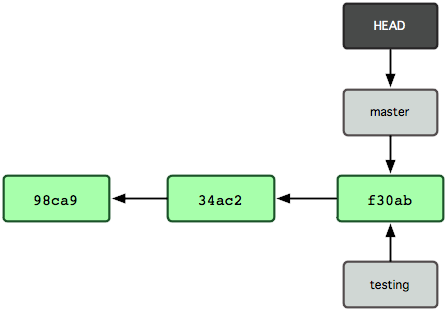
\includegraphics[width=8cm]{git-branch-create}
  \caption{分支建立后}\label{git-branch-create}
\end{figure}

删除一个分支也很简单,只要加上-d选项(-D是强制删除)即可,就像这样

\begin{minted}[linenos]{bash}
# 创建一个基于当前分支产生的分支,其名字为<branch-name>
$ git branch -d(D) <branch-name>
\end{minted}

想查看分支情况以及当前所在分支,只需要加上 -a选项即可

\begin{minted}[linenos]{bash}
# 查看所有的远程与本地分支
$ git branch -a

# 使用该命令的效果如下
# 前面带*的分支是当前分支
  lab1
  lab1-exam
* lab1-result
  master
  remotes/origin/HEAD -> origin/master
  remotes/origin/lab1
  remotes/origin/lab1-exam
  remotes/origin/lab1-result
  remotes/origin/master
# 带remotes是远程分支,在后面提到远程仓库的时候我们会知道
\end{minted}

我们建立了分支并不代表会自动切换到分支,那么,Git 是如何知道你当前在哪个分支上工作的呢?其实答案也很简单,它保存着一个名为HEAD的特别指针。在 Git 中,它是一个指向你正在工作中的本地分支的指针,可以将 HEAD 想象为当前分支的别名。运行git branch 命令,仅仅是建立了一个新的分支,但不会自动切换到这个分支中去,所以在这个例子中,我们依然还在 master 分支里工作。

那么我们如何切换到另一个分支去呢,这时候我们就要用到这个我们在实验中更常见的分支指令了\label{git checkout}
\begin{minted}[linenos]{bash}
# 切换到<branch-name>代表的分支,这时候HEAD游标指向新的分支
$ git checkout <branch-name>
\end{minted}

比如这时候我们使用 \textbf{git checkout testing},这样 HEAD 就指向了 testing 分支(见图\ref{git-branch-checkout})。

\begin{figure}[htbp]
  \centering
  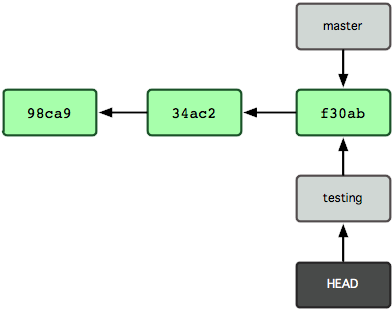
\includegraphics[width=8cm]{git-branch-checkout}
  \caption{分支切换后}\label{git-branch-checkout}
\end{figure}

这时候你会发现你的工作区就是testing分支下的工作目录,而且在testing分支下的修改,添加与提交不会对master分支产生任何影响。

在我们的操作系统实验中,有以下几种分支:
\begin{description}
\item[labx] 这是我们提交实验代码的分支,这个分支不需要我们手动创建。当写好代码提交到服务器上后,在该次实验结束后,使用后面提到的\hyperref[更新指令]{更新指令}可获取到新的实验分支,到时只需要使用git checkout labx即可进行新的实验。
\item[labx-exam] 这是我们周一小测实验的分支,每次需要使用 git branch 指令将刚完成的实验分支拷贝一份到 labx-exam分支下,并进行小测代码的填写。
\item[labx-result] 这是我们每次实验结果的分支,每次的实验结果将会在该分支工作区的 log 文件夹下,数字越大代表检测的时间越近。测试下方Summary : Number (in 100),只要Number >= 60即算作通过本次实验。
\end{description}

\begin{note}
每次实验虽然是60算实验通过,但是Summary最好是100。因为每次新实验的代码是你刚完成的实验代码以及一些新的要填充的文件组成的,前面实验的错误可能会在后面的实验中变成不小的坑。当然Summary为100也不代表实验一定全部正确,尽可能多花点时间理解与修改。
\end{note}

我们之前所介绍的这些指令只是在本地进行操作的,其中必须掌握

\begin{enumerate}
  \item \hyperref[git add]{git add}
  \item \hyperref[git commit]{git commit}
  \item \hyperref[git branch]{git branch}
  \item \hyperref[git checkout]{git checkout}
\end{enumerate}

其余指令可以临时查阅,当然掌握对你益处现在体会不出来,但当你们小团队哪天一起做项目的时候,你就会体会到掌握这么多Git的知识是件多么幸福的事情了。之前我们所有的操作都是在本地版本库上操作的,下面我们要介绍的是一组和远程仓库有关的
指令。这组指令是最容易出错的,所以你一定要认真学习。

\subsection{Git远程仓库与本地}

在我们的实验中,我们设立了几台服务器主机作为大家的远程仓库。那么远程仓库是什么呢?远程仓库其实和你本地版本库结构是一致的,只不过远程仓库是在服务器上的仓库,而本地仓库是在本地的。实验中我们每次对代码有所修改时,最后都需要在实验截止时间之前提交到服务器上,我们以服务器上的远程仓库里的代码为评测标准哦。我们先介绍一条我们实验中比较常用的一条命令

\begin{minted}[linenos]{bash}
# git clone 用于从远程仓库克隆一份到本地版本库
$ git clone git@ip:学号-lab
\end{minted}

从名字也能很容易理解这条指令的含义所在,我们就是使用clone指令而把服务器上的远程仓库拷贝到本地版本库里。这是一条很重要的指令,以后我们会经常使用。包括前期检查我们是否成功地提交到服务器上,以及后期使用Git为开源社区做贡献时都需要。但是初学者在使用这条命令的时候可能会遇到一个问题,那么来仔细思考一下下面的问题\par

\begin{thinking}\label{think-克隆}
思考下面四个描述,你觉得哪些正确,哪些错误,请给出你参考的资料或实验证据。
\begin{enumerate}
  \item 克隆时所有分支均被克隆,但只有HEAD指向的分支被检出。
  \item 克隆出的工作区中执行 git log、git status、git checkout、git commit等操作不会去访问远程版本库。
  \item 克隆时只有远程版本库HEAD指向的分支被克隆。
  \item 克隆后工作区的默认分支处于master分支。
\end{enumerate}
\end{thinking}

\begin{note}
检出某分支指的是在该分支有对应的本地分支,使用git checkout 后会在本地检出一个同名分支自动跟踪远程分支。比如现在本地空无一物,远程有一个名为 os的分支,我们使用 git checkout os 即可在本地建立一个跟远程分支同名,自动追踪远程分支的os分支,并且在os分支下push时会默认提交到远程分支 os上。
\end{note}

初学者最容易犯的一个错误是,在检查自己是否提交到服务器上时,克隆下来就着急忙慌地编译。大侠莫慌,看清楚分支再编译。我们克隆下来时默认处于master分支,但很可惜实验的代码是不会在master分支上测试的,所以我们要先使用\hyperref[git checkout]{git checkout}检出对应的labx分支,再进行测试。

下面再介绍两条跟远程仓库有关的指令,其作用很简单,但要用好却是比较难。
\begin{minted}[linenos]{bash}
# git push 用于从本地版本库推送到服务器远程仓库
$ git push

# git pull 用于从服务器远程仓库抓取到本地版本库
$ git pull
\end{minted}
git push只是将本地版本库里已经commit的部分同步到服务器上去,不包括\textbf{暂存区}里存放的内容。在我们实验中除了还可能会加些选项使用

\begin{minted}[linenos]{bash}
# origin在我们实验里是固定的,以后就明白了。branch是指本地分支的名称。
$ git push origin [branch]
\end{minted}

这条指令可以将我们本地创建的分支推送到远程仓库中,在远程仓库建立一个同名的本地追踪的远程分支。比如我们实验小测时要在本地先建立一个\textbf{labx-exam}的分支,在提交完成后,我们要使用\textbf{git push origin labx-exam}在服务器上建立一个同名远程分支,这样服务器才可以通过检测该分支的代码来检测你的代码是否正确。

git pull\label{更新指令} 是条更新用的指令,如果助教老师在服务器端发布了新的分支,下发了新的代码或者进行了一些改动的话,我们就需要使用 git pull来让本地版本库与远程仓库保持同步。

\subsection{Git冲突与解决冲突}

这两条指令含义注释里也写得清楚,但是还是很容易出问题。新手使用push时,容易出现的大问题会是这样的

\begin{minted}[linenos]{bash}
中文版:
To git@github.com:1406xxxx.git
 ! [rejected]        master -> master (non-fast-forward) 
error: 无法推送一些引用到 'git@github.com:1406xxxx.git' 
提示:更新被拒绝,因为您当前分支的最新提交落后于其对应的远程分支。 
提示:再次推送前,先与远程变更合并(如 'git pull ...')。详见 
提示:'git push --help' 中的 'Note about fast-forwards' 小节。

英文版:
To git@github.com:1406xxxx.git
 ! [rejected]        master -> master (non-fast-forward)
error: failed to push some refs to 'To git@github.com:1406xxxx.git'
hint: Updates were rejected because the tip of your current branch is behind
hint: its remote counterpart. Integrate the remote changes (e.g.
hint: 'git pull ...') before pushing again.
hint: See the 'Note about fast-forwards' in 'git push --help' for details.
\end{minted}

你的提示可能是英文的,但这并不妨碍问题的发生,这个问题是因为什么而产生的呢?我们来分析一下,想象你在公司和在家操作同一个分支,在公司你对一个文件进行了修改,然后进行了提交。回了家又对同样的文件做了不同的修改,在家中使用push同步到远程分支了。但等你回到公司再push的时候就会发现一个严重的问题:现在远程仓库和本地仓库已经分离开变成两条岔路了(见图\ref{git-remote-branches})。

\begin{figure}[htbp]
  \centering
  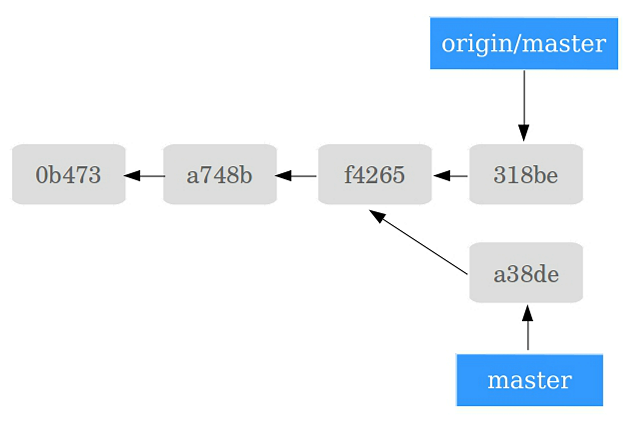
\includegraphics[width=10cm]{git-remote-branches}
  \caption{远程仓库与本地仓库的岔路}\label{git-remote-branches}
\end{figure}

这样的话远程仓库可就为难了,你在公司的提交有效,在家里的提交也有效,你又不想浪费劳动成果,想让远程仓库把你的提交全部接受,那么我们怎么样才能解决这个问题呢?这时候就要请出我们的\textbf{git pull}指令了!

你此时可能会产生一个很大的疑问,在push之前,使用git pull轻轻一挥,难道问题就能全部解决?答案当然是否定的,我们不能指望Git帮我们把文件中的修改全部妥善合并,但是Git为我们提供了另一种机制帮我们能快速定位有冲突(conflict)的文件,这时候我们使用git pull,你可能会看到有下面这样的提示

\begin{minted}[linenos]{bash}
Auto-merging test.txt
CONFLICT (content): Merge conflict in test.txt
Automatic merge failed; fix conflicts and then commit the result.
\end{minted}

有冲突的文件中往往包含一部分类似如下的奇怪代码,我们打开test.txt,发现这样一些“乱码”

\begin{minted}[linenos]{bash}

a123
<<<<<<< HEAD
b789
=======
b45678910
>>>>>>> 6853e5ff961e684d3a6c02d4d06183b5ff330dcc
c
\end{minted}

冲突标记\verb|<<<<<<<| 与=======之间的内容是你在家里的修改,=======与\verb|>>>>>>>|之间的内容是你在公司的修改。

要解决冲突也很简单:编辑冲突文件,将其中冲突的内容手工合理合并一下就可以了,当然记得在文件中解决了冲突之后要重新add该文件并commit。大声告诉我,是不是非常简单?

然而世间并没有那么多简单的事情,如果你足够不幸,你可能在git pull的时候也会遇到不小的问题,问题可能是这样的

\begin{minted}[linenos]{bash}
error: Your local changes to the following files would be overwritten by merge:
	1406xxxx-lab/readme.txt
Please, commit your changes or stash them before you can merge.
Aborting
\end{minted}

其实提示已经比较清楚了,这里我们只需要把我们之前的所有修改全部提交(commit)即可,提交之后再git pull就好。当然,有更高级的用法是这样的,不推荐大家现在学习,如果你已经熟悉了Git的基础操作,那么可以阅读\href{http://www.01happy.com/git-resolve-conflicts/}{git stash解决git pull冲突}

不要觉得这一节的冲突一节不需要学习,因为你可能会想:我现在怎么可能在公司和家里同时修改文件呢!但是要注意,在远程仓库编辑的不止你一个人,还有助教老师,助教老师一旦修改一些东西都有可能产生冲突,所以你一定要认真学会这一节的内容。当然实践是最好的老师,我们再来实践一下

\begin{exercise}
仔细回顾一下上面这些指令,然后完成下面的任务
  \begin{itemize}
    \item 在 /home/1406xxxx/1406xxxx-lab下新建分支,名字为Test
    \item 切换到Test分支,添加一份readme.txt,内容写入自己的学号
    \item 将文件提交到本地版本库,然后建立相应的远程分支。
  \end{itemize}
\end{exercise}

到这里Git教程基本就算是结束了,能看完这么长的教程也真是辛苦你了,奉送一下实验代码提交流程的简明教程,希望你可以快速上手,终身难忘!

\subsection{实验代码提交流程}

\begin{description}
\item[modify] 写代码。
\item[git add & git commit <modified-file>] 提交到本地版本库。
\item[git pull] 从服务器拉回本地版本库,并解决服务器版本库与本地代码的冲突。
\item[git add & git commit <conflict-file>] 将远程库与本地代码合并结果提交到本地版本库。
\item[git push] 将本地版本库推到服务器。
\item[mkdir test & cd test & git clone] 建立一个额外的文件夹来测试服务器上的代码是否正确。
\end{description}

而我们在一次实验结束,新的实验代码下发时,一般是按照以下流程的来开启新的实验之旅。

\begin{description}
\item[git add & git commit] 如果当前分支的暂存区还有东西的话,先提交。
\item[git pull] 这一步很重要!要先确保服务器上的更新全部同步到本地版本库!
\item[git checkout labx] 检出新实验分支并进行实验。
\end{description}

谨记,一定要勤使用\textbf{git pull},这条指令很重要!有事没事,同步一下!

感谢你看这篇长长的Git教程到现在,希望你能快乐地使用Git,若有不会勤查教程\footnote{推荐廖雪峰老师的网站:
\url{http://www.liaoxuefeng.com/}}。如果你希望能学到更厉害的技术,推荐\href{https://github.com/Gazler/githug}{GitHug},这是一个关于Git的通关小游戏。开启你快乐的实验之旅吧!\verb|^_^|

\section{实验思考}
\begin{itemize}
\item \hyperref[think-小明的困境]{\textbf{\textcolor{baseB}{思考-小明的困境}}}
\item \hyperref[think-克隆]{\textbf{\textcolor{baseB}{思考-克隆命令}}}
\end{itemize}

请认真做练习,然后把实验思考里的内容附在实验文档中一起提交!